\documentclass[dvipdfmx,cjk,10.2pt]{beamer} 
%\documentclass[dvipdfm,cjk]{beamer} %% オプションは環境や利用するプログラムに
%\documentclass[dvips,cjk]{beamer}   %% よって変える

\usepackage{subfigure}
\usepackage[all]{xy}
\usepackage{wrapfig}

\newcommand{\C}{\mathbb{C}}
\newcommand{\D}{\mathbb{D}}
\newcommand{\R}{\mathbb{R}}
\newcommand{\Q}{\mathbb{Q}}
\newcommand{\Z}{\mathbb{Z}}
\newcommand{\N}{\mathbb{N}}

\newcommand{\Imag}{\mathrm{Im}}
\newcommand{\id}{\mathrm{id}}


\makeatletter
\newcommand\xleftrightarrow[2][]{%
  \ext@arrow 9999{\longleftrightarrowfill@}{#1}{#2}}
\newcommand\longleftrightarrowfill@{%
  \arrowfill@\leftarrow\relbar\rightarrow}
\makeatother

\AtBeginDvi{\special{pdf:tounicode 90ms-RKSJ-UCS2}} %% しおりが文字化けしないように
%\AtBeginDvi{\special{pdf:tounicode EUC-UCS2}}

\setbeamertemplate{navigation symbols}{} %% 右下のアイコンを消す
\setbeamertemplate{theorems}[normal font] %%斜体を直す

\usetheme{CambridgeUS}         %% theme の選択
%\usetheme{Boadilla}           %% Beamer のディレクトリの中の
%\usetheme{Madrid}             %% beamerthemeCambridgeUS.sty を指定
%\usetheme{Antibes}            %% 色々と試してみるといいだろう
%\usetheme{Montpellier}        %% サンプルが beamer\doc に色々とある。
%\usetheme{Berkeley}
%\usetheme{Goettingen}
%\usetheme{Singapore}
%\usetheme{Szeged}

%\usecolortheme{rose}          %% colortheme を選ぶと色使いが変わる
%\usecolortheme{albatross}

%\useoutertheme{shadow}                 %% 箱に影をつける
\usefonttheme{professionalfonts}       %% 数式の文字を通常の LaTeX と同じにする

%\setbeamercovered{transparent}         %% 消えている文字をうっすらと表示する


\theoremstyle{definition}
\setbeamertemplate{theorems}[numbered]  %% 定理に番号をつける
\newtheorem{Thm}{定理}[section]
%\theoremstyle{example}
\newtheorem{Ex}[Thm]{例}
%\newtheorem{exam}[thm]{Example}
\newtheorem{Rem}[Thm]{注意}
\newtheorem{Conj}[Thm]{予想}
\newtheorem{Def}[Thm]{定義}
\newtheorem{Prob}[Thm]{問題}

\setbeamercolor{block title}{fg=blue!70!black, bg=blue!15!white} 
\setbeamercolor{block body}{fg=black, bg=blue!10!white}



\begin{document}
\title{微分・積分 第3回} 
\author{慶応義塾大学}            %% ここに書かれた情報は色々なところに使われるので
\institute[]{総合政策学部・環境情報学部}   %% なるべく設定した方が良い
\date{}



\begin{frame}                  %% \begin{frame}..\end{frame} で 1 枚のスライド
\titlepage                     %% タイトルページ
\end{frame}

%\begin{frame}                  %% 目次 (必要なければ省略)
%\tableofcontents
%\end{frame}






%%%%%%%%%%%%%%%%%%%%%%%%%%%%%%%%%%%%%%%%%%%%%%%%%%%%%%%%%%%%%%%%%%%%%%%%%%%%%%%%%%%%%%%
%%%%%%%%%%%%%%%%%%%%%%%%%%%%%%%%%%%%%%%%%%%%%%%%%%%%%%%%%%%%%%%%%%%%%%%%%%%%%%%%%%%%%%%

\section{講義概要}


\begin{frame}
\frametitle{今日の内容}



\begin{enumerate}
\item 極限 (右極限, 左極限, 極限, 極限の性質)
\item 連続 (点連続, 連続関数, 中間値の定理)
\item 不定形の極限
\end{enumerate} 



\end{frame}






%%%%%%%%%%%%%%%%%%%%%%%%%%%%%%%%%%%%%%%%%%%%%%%%%%%%%%%%%%%%%%%%%%%%%%%%%%%%%%%%%%%%%%%
%%%%%%%%%%%%%%%%%%%%%%%%%%%%%%%%%%%%%%%%%%%%%%%%%%%%%%%%%%%%%%%%%%%%%%%%%%%%%%%%%%%%%%%

\section{極限}

\begin{frame}
\frametitle{極限}



\begin{itemize}
\item 除法において, $0$で割ることは出来ない. $1/0$や$0/0$は存在しない. 
\item 無限大$\infty$と言う数は存在しない. $\infty-10$, $1/\infty$, $\infty - \infty$などは意味を持たない. 
\item しばしば, $1/0$, $1/\infty$, $\infty - \infty$などに近いものを扱う必要がある.
\begin{itemize}
\item 微分: 微小変化($0/0$に近いもの)を評価する. 
\item 積分: 微小量の無限和($\infty \times 0$に近いもの)を評価する. 
\end{itemize}
このようなものを数学的に適切に扱うために, ``極限"の概念が必要になる. 
\end{itemize}

\end{frame}





%%%%%%%%%%%%%%%%%%%%%%%%%%%%%%%%%%%%%%%%%%%%%%%%%%%%%%%%%%%%%%%%%%%%%%%%%%%%%%%%%%%%%%%
%%%%%%%%%%%%%%%%%%%%%%%%%%%%%%%%%%%%%%%%%%%%%%%%%%%%%%%%%%%%%%%%%%%%%%%%%%%%%%%%%%%%%%%


\begin{frame}
\frametitle{右極限, 左極限}

関数の値の``極限"を考えたい. 

\begin{itemize}
\item 例えば, 関数$1/x$は原点$0$では定義されないが, 原点の近傍では定義されている. 
\item $x>0$の方から原点に近付くと, 関数の値は正の値で発散, つまり$+\infty$になる. 
\item 一方で, $x<0$の方から原点に近付くと, 関数の値は負の値で発散, つまり$-\infty$になる. 
\end{itemize}

\vspace{-1mm}

 \begin{figure}[htbp]
 \begin{center} 
  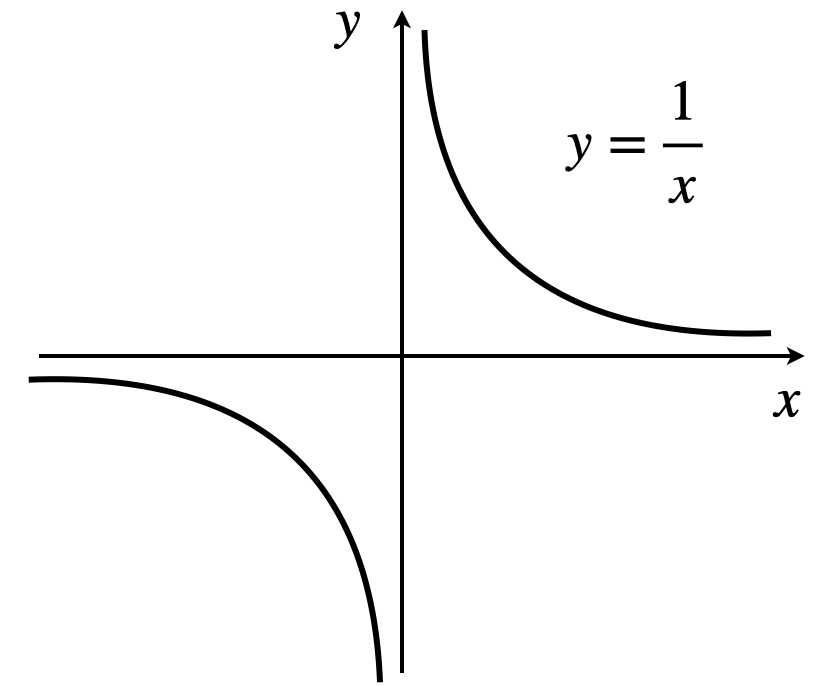
\includegraphics[width=40mm]{xinv.png}
 \end{center}
\end{figure}

\vspace{-1mm}

\end{frame}



%%%%%%%%%%%%%%%%%%%%%%%%%%%%%%%%%%%%%%%%%%%%%%%%%%%%%%%%%%%%%%%%%%%%%%%%%%%%%%%%%%%%%%%
%%%%%%%%%%%%%%%%%%%%%%%%%%%%%%%%%%%%%%%%%%%%%%%%%%%%%%%%%%%%%%%%%%%%%%%%%%%%%%%%%%%%%%%

\section{片側極限}

\begin{frame}
\frametitle{右極限}

\begin{Def}
関数$f(x)$に関して, $x > a$を満たしながら$x$が$a$に近付くとき
\begin{itemize}
\item $f(x)$が$\alpha \in \R$に収束することを次のように表す. 
$$
\lim_{x \to a +0} f(x)=\alpha, 
$$
\item $f(x)$がいくらでも大きく(小さく)なることを, 正(負)の無限大に発散するといい,次のように表す. 
$$
\lim_{x \to a +0} f(x)=+\infty \ (-\infty)
$$
\end{itemize}
これらを$f(x)$の$a$における\underline{右極限}という. 
\end{Def}

$a=0$の場合は特別で, $x \to 0+0$と書かずに, $x\to +0$と書く. 

\end{frame}


%%%%%%%%%%%%%%%%%%%%%%%%%%%%%%%%%%%%%%%%%%%%%%%%%%%%%%%%%%%%%%%%%%%%%%%%%%%%%%%%%%%%%%%
%%%%%%%%%%%%%%%%%%%%%%%%%%%%%%%%%%%%%%%%%%%%%%%%%%%%%%%%%%%%%%%%%%%%%%%%%%%%%%%%%%%%%%%


\begin{frame}
\frametitle{左極限}

\begin{Def}
関数$f(x)$に関して, $x < a$を満たしながら$x$が$a$に近付くとき
\begin{itemize}
\item $f(x)$が$\alpha \in \R$に収束することを次のように表す. 
$$
\lim_{x \to a -0} f(x)=\alpha, 
$$
\item $f(x)$がいくらでも大きく(小さく)なることを, 正(負)の無限大に発散するといい, 次のように表す. 
$$
\lim_{x \to a -0} f(x)=+\infty \ (-\infty)
$$
\end{itemize}
これらを$f(x)$の$a$における\underline{左極限}という. 
\end{Def}

$a=0$の場合は特別で, $x \to 0-0$と書かずに, $x\to -0$と書く. 

\end{frame}

%%%%%%%%%%%%%%%%%%%%%%%%%%%%%%%%%%%%%%%%%%%%%%%%%%%%%%%%%%%%%%%%%%%%%%%%%%%%%%%%%%%%%%%
%%%%%%%%%%%%%%%%%%%%%%%%%%%%%%%%%%%%%%%%%%%%%%%%%%%%%%%%%%%%%%%%%%%%%%%%%%%%%%%%%%%%%%%


\begin{frame}
\frametitle{片側極限}

\begin{itemize}
\item 右極限と左極限は\underline{片側極限}とも呼ばれる. 
\item 関数$f(x)$の$a$における右極限と左極限は一般に一致しない. 
\item $f(a)$は定義されるとは限らないし, 定義されても極限と一致するとは限らない. 
\end{itemize}
例: $f(x)=\frac{1}{x}$, \vspace{-2mm}
$$
\lim_{x \to +0}\frac{1}{x}= +\infty, \ \ \ \lim_{x \to -0}\frac{1}{x}=-\infty
$$

\vspace{-3mm}

 \begin{figure}[htbp]
 \begin{center} 
  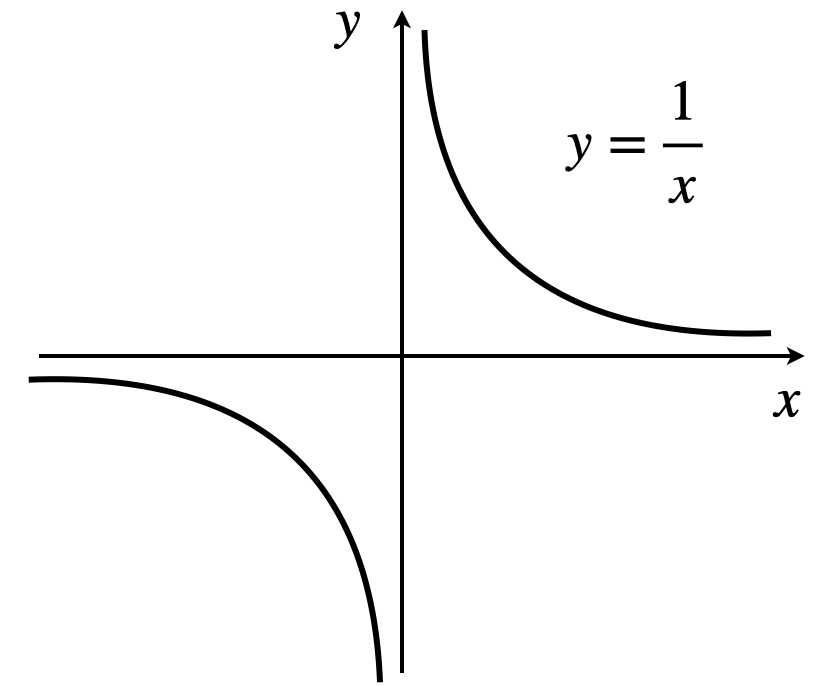
\includegraphics[width=40mm]{xinv.png}
 \end{center}
\end{figure}

\vspace{-3mm}

\end{frame}





%%%%%%%%%%%%%%%%%%%%%%%%%%%%%%%%%%%%%%%%%%%%%%%%%%%%%%%%%%%%%%%%%%%%%%%%%%%%%%%%%%%%%%%
%%%%%%%%%%%%%%%%%%%%%%%%%%%%%%%%%%%%%%%%%%%%%%%%%%%%%%%%%%%%%%%%%%%%%%%%%%%%%%%%%%%%%%%


\begin{frame}
\frametitle{片側極限}


例: $\mathrm{sgn}(0)=0$, 
$$
\lim_{x \to +0}\mathrm{sgn}(x)=1, \ \ \ \lim_{x \to -0}\mathrm{sgn}(x)=-1
$$

\vspace{-3mm}

 \begin{figure}[htbp]
 \begin{center} 
  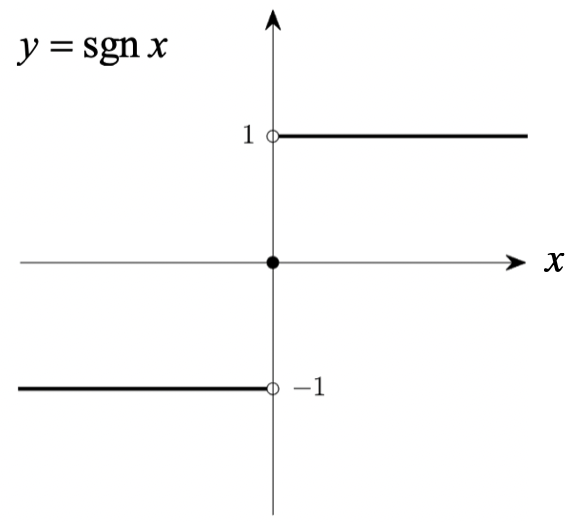
\includegraphics[width=45mm]{sgn.png}
 \end{center}
\end{figure}

\vspace{-3mm}

\end{frame}




%%%%%%%%%%%%%%%%%%%%%%%%%%%%%%%%%%%%%%%%%%%%%%%%%%%%%%%%%%%%%%%%%%%%%%%%%%%%%%%%%%%%%%%
%%%%%%%%%%%%%%%%%%%%%%%%%%%%%%%%%%%%%%%%%%%%%%%%%%%%%%%%%%%%%%%%%%%%%%%%%%%%%%%%%%%%%%%

\section{極限}

\begin{frame}
\frametitle{極限} 


\begin{Def}
関数$f(x)$の$a$における右極限と左極限が存在し, それらが一致するとき, その値を
$$
\lim_{x\to a} f(x)
$$
と書いて, $f(x)$の$a$における\underline{極限}という. 
\end{Def}

つまり$x$が$a$にどのような近付き方をしても, その値が曖昧なく定まるときに極限が定義される. 
定義より, 極限が存在するとき
$$
\lim_{x\to a} f(x) = \lim_{x\to a+0} f(x) = \lim_{x\to a-0} f(x). 
$$

\end{frame}


%%%%%%%%%%%%%%%%%%%%%%%%%%%%%%%%%%%%%%%%%%%%%%%%%%%%%%%%%%%%%%%%%%%%%%%%%%%%%%%%%%%%%%%
%%%%%%%%%%%%%%%%%%%%%%%%%%%%%%%%%%%%%%%%%%%%%%%%%%%%%%%%%%%%%%%%%%%%%%%%%%%%%%%%%%%%%%%


\begin{frame}
\frametitle{極限} 


\begin{itemize}
\item 右極限と左極限が一致しないので, 極限
$$
\lim_{x\to 0}\frac{1}{x}, \ \ \ \lim_{x\to0}\mathrm{sgn}(x)
$$
は存在しない. 
\item 一方で, 
$$
\lim_{x\to +0}\frac{1}{|x|}=\lim_{x\to -0}\frac{1}{|x|}=+\infty
$$
であるから, 極限が存在して
$$
\lim_{x\to 0}\frac{1}{|x|}=\infty. 
$$
\end{itemize}

\end{frame}


%%%%%%%%%%%%%%%%%%%%%%%%%%%%%%%%%%%%%%%%%%%%%%%%%%%%%%%%%%%%%%%%%%%%%%%%%%%%%%%%%%%%%%%
%%%%%%%%%%%%%%%%%%%%%%%%%%%%%%%%%%%%%%%%%%%%%%%%%%%%%%%%%%%%%%%%%%%%%%%%%%%%%%%%%%%%%%%


\begin{frame}
\frametitle{極限} 



\begin{Prob}
\begin{itemize}
\item $\displaystyle \lim_{x\to +0}|x|$, $\displaystyle \lim_{x\to -0}|x|$を求めよ. 
\item $\displaystyle \lim_{x\to0}|x|$は存在するか? 
\end{itemize}
\end{Prob}


\begin{Prob}
\begin{itemize}
\item $\displaystyle \lim_{x\to +0}\mathrm{sgn}(|x|)$,  $\displaystyle \lim_{x\to -0}\mathrm{sgn}(|x|)$を求めよ. 
\item $\displaystyle \lim_{x\to 0}\mathrm{sgn}(|x|)$は存在するか? 
\end{itemize}
\end{Prob}

\begin{Prob}
\begin{itemize}
\item $\displaystyle \lim_{x\to +0}(x^2-x)/|x|$,   $\displaystyle \lim_{x\to -0}(x^2-x)/|x|$を求めよ. 
\item $\displaystyle \lim_{x\to 0} (x^2-x)/|x|$は存在するか? 
\end{itemize}
\end{Prob}

\end{frame}



%%%%%%%%%%%%%%%%%%%%%%%%%%%%%%%%%%%%%%%%%%%%%%%%%%%%%%%%%%%%%%%%%%%%%%%%%%%%%%%%%%%%%%%
%%%%%%%%%%%%%%%%%%%%%%%%%%%%%%%%%%%%%%%%%%%%%%%%%%%%%%%%%%%%%%%%%%%%%%%%%%%%%%%%%%%%%%%


\begin{frame}
\frametitle{注意事項} 


\begin{Rem}
\begin{itemize}
\item ``$x$が$a$に近付くときに, $f(x)$が$\alpha$に収束する"を厳密に定義するには, $\epsilon$-$\delta$論法を用いる必要があるが, この講義では扱わない. 
\item $1/x$の例からも分かるように, $x$の近付く先$a$が定義域に含まれている必要はない. 
つまり$f(a)$が定義されていなくても, $\displaystyle \lim_{x \to a+0}f(x)$などの極限は議論できる. 
\item 一方で, $a$が$f$の定義域$D$内の点で近似できないと$f(x)$の$a$における極限は定義できない. 
つまり, $a$は$D$もしくはその境界$\partial D$に含まれる必要がある. (閉包$\overline{D}$: $D$と$\partial D$の集合)
\end{itemize}
\end{Rem}

本講義は入門的な位置付けなので, 厳密性にはあまり拘らないで議論を進める. 

\end{frame}



%%%%%%%%%%%%%%%%%%%%%%%%%%%%%%%%%%%%%%%%%%%%%%%%%%%%%%%%%%%%%%%%%%%%%%%%%%%%%%%%%%%%%%%
%%%%%%%%%%%%%%%%%%%%%%%%%%%%%%%%%%%%%%%%%%%%%%%%%%%%%%%%%%%%%%%%%%%%%%%%%%%%%%%%%%%%%%%


\begin{frame}
\frametitle{極限の性質} 


\begin{Thm}
$\displaystyle \lim_{x\to a}f(x)=\alpha$, $\displaystyle \lim_{x\to a}g(x)=\beta$で$\alpha,\beta \in \R$とする. 
このとき
\begin{itemize}
\item $\displaystyle \lim_{x\to a} cf(x)=c \alpha$, \vspace{1mm}
\item $\displaystyle \lim_{x\to a}(f(x)+g(x))=\alpha+\beta$, \ $\displaystyle \lim_{x\to a}f(x)g(x)=\alpha\beta$,  \vspace{1mm}
\item $\beta \neq0$であれば, $\displaystyle \lim_{x\to a}f(x)/g(x)=\alpha/\beta$,  \vspace{1mm}
\item $a$の近傍で$f(x)\le g(x)$であれば, $\alpha \le \beta$, 
\end{itemize}
\end{Thm}

最後の主張は少し注意が必要で, $a$の近傍で$f(x)< g(x)$であっても$\alpha < \beta$とは限らない.  
($f(x)< g(x)$であれば$f(x)\le g(x)$なので, $\alpha \le \beta$は正しい.)

\end{frame}


%%%%%%%%%%%%%%%%%%%%%%%%%%%%%%%%%%%%%%%%%%%%%%%%%%%%%%%%%%%%%%%%%%%%%%%%%%%%%%%%%%%%%%%
%%%%%%%%%%%%%%%%%%%%%%%%%%%%%%%%%%%%%%%%%%%%%%%%%%%%%%%%%%%%%%%%%%%%%%%%%%%%%%%%%%%%%%%


%\begin{frame}
%\frametitle{極限の性質} 
%
%
%\begin{Thm}
%$\lim_{x\to a}|f(x)|=+\infty$であれば, $\lim_{x\to a}1/f(x)=0$. 
%\end{Thm}
%定理において, $a=\pm \infty$でも構わない. 
%
%
%\end{frame}



%%%%%%%%%%%%%%%%%%%%%%%%%%%%%%%%%%%%%%%%%%%%%%%%%%%%%%%%%%%%%%%%%%%%%%%%%%%%%%%%%%%%%%%
%%%%%%%%%%%%%%%%%%%%%%%%%%%%%%%%%%%%%%%%%%%%%%%%%%%%%%%%%%%%%%%%%%%%%%%%%%%%%%%%%%%%%%%


\begin{frame}
\frametitle{極限の性質} 


\begin{Prob}
次を計算せよ. 
\begin{itemize}
\item $\displaystyle \lim_{x\to 1} (x^2+3x+5)$
\item $\displaystyle \lim_{x\to 0} (2x+5)\mathrm{sgn}(|x|)$
\end{itemize}
\end{Prob}

\begin{Prob} 
$0$の近傍で$f(x)< g(x)$であり, $\displaystyle \lim_{x\to 0}f(x) = \lim_{x\to 0}g(x)$なる関数$f(x),g(x)$を1つ見つけよ.
\end{Prob}


\end{frame}




%%%%%%%%%%%%%%%%%%%%%%%%%%%%%%%%%%%%%%%%%%%%%%%%%%%%%%%%%%%%%%%%%%%%%%%%%%%%%%%%%%%%%%%
%%%%%%%%%%%%%%%%%%%%%%%%%%%%%%%%%%%%%%%%%%%%%%%%%%%%%%%%%%%%%%%%%%%%%%%%%%%%%%%%%%%%%%%


\begin{frame}
\frametitle{極限の性質} 


これまでは$a \in \R$に対して極限$\displaystyle \lim_{x \to a}f(x)$を考えていたが, $a= \pm \infty$に対しても同様の議論が可能である. 
次の定義は厳密には不十分であるが, この講義では特に問題にならない.  

\begin{itemize}
\item $x$が十分大きくなるとき, $f(x)$が$\alpha$に収束することを
$$
\lim_{x\to +\infty} f(x)=\alpha, 
$$
\item $x$が十分小さくなるとき, $f(x)$が$\alpha$に収束することを
$$
\lim_{x\to -\infty} f(x)=\alpha
$$
\end{itemize}
と書く. 

\end{frame}




%%%%%%%%%%%%%%%%%%%%%%%%%%%%%%%%%%%%%%%%%%%%%%%%%%%%%%%%%%%%%%%%%%%%%%%%%%%%%%%%%%%%%%%
%%%%%%%%%%%%%%%%%%%%%%%%%%%%%%%%%%%%%%%%%%%%%%%%%%%%%%%%%%%%%%%%%%%%%%%%%%%%%%%%%%%%%%%

\section{連続}

\begin{frame}
\frametitle{連続} 


\begin{Def}
\begin{itemize}
\item $f(x)$が\underline{$a$で連続}であるとは, 
$$
\lim_{x\to a}f(x)=f(a)
$$
が成立すること. 
つまり, 極限$\displaystyle \lim_{x\to a}f(x)$が存在し, $f(a) \in \R$が定義され, それらが一致すること. 
連続でないとき, \underline{不連続}という. 
\item $f(x)$が\underline{連続関数}であるとは, 定義域の全ての点において連続であること. 
\end{itemize}
\end{Def}

$f(x)$が$a$で連続であるとき, $\displaystyle \lim_{x\to a}f(x) \neq \pm  \infty$であることに注意. 

\end{frame}



%%%%%%%%%%%%%%%%%%%%%%%%%%%%%%%%%%%%%%%%%%%%%%%%%%%%%%%%%%%%%%%%%%%%%%%%%%%%%%%%%%%%%%%
%%%%%%%%%%%%%%%%%%%%%%%%%%%%%%%%%%%%%%%%%%%%%%%%%%%%%%%%%%%%%%%%%%%%%%%%%%%%%%%%%%%%%%%


\begin{frame}
\frametitle{不連続} 



\begin{itemize}
\item  $1/x$や$\mathrm{sgn}(x)$は$0$において不連続. ($x\neq 0$では連続である.) 
\item $1/|x|$は$1/|0|$が定義されないから, $0$において不連続. ($\displaystyle \lim_{x\to 0}1/|x|=+\infty$でもある.)
\end{itemize}


%\vspace{-1mm}

 \begin{figure}[htbp]
 \begin{center} 
  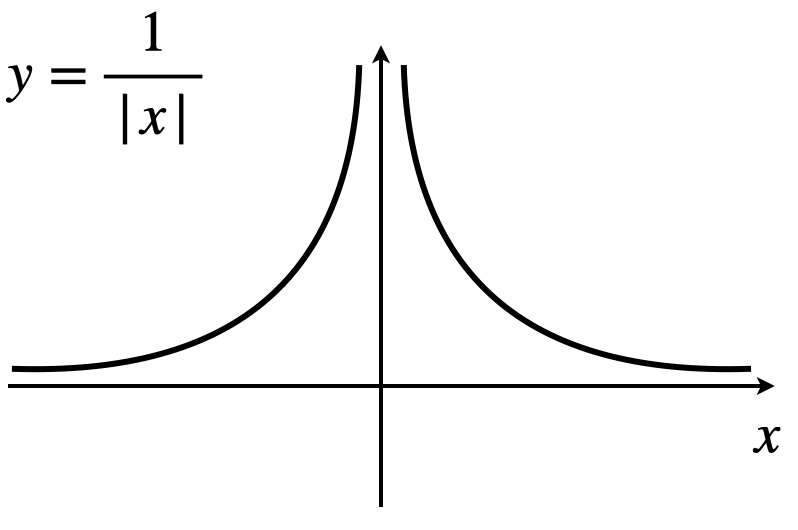
\includegraphics[width=50mm]{xinv_abs.png}
 \end{center}
\end{figure}

\vspace{-1mm}


\end{frame}



%%%%%%%%%%%%%%%%%%%%%%%%%%%%%%%%%%%%%%%%%%%%%%%%%%%%%%%%%%%%%%%%%%%%%%%%%%%%%%%%%%%%%%%
%%%%%%%%%%%%%%%%%%%%%%%%%%%%%%%%%%%%%%%%%%%%%%%%%%%%%%%%%%%%%%%%%%%%%%%%%%%%%%%%%%%%%%%


\begin{frame}
\frametitle{不連続} 



$\mathrm{sgn}(|x|)$は, 極限$\displaystyle \lim_{x\to 0}\mathrm{sgn}(|x|)$が存在し, $\mathrm{sgn}(|0|)$も定義されるが
$$
\lim_{x\to 0}\mathrm{sgn}(|x|) \neq  \mathrm{sgn}(|0|).
$$ 

\vspace{-1mm}

 \begin{figure}[htbp]
 \begin{center} 
  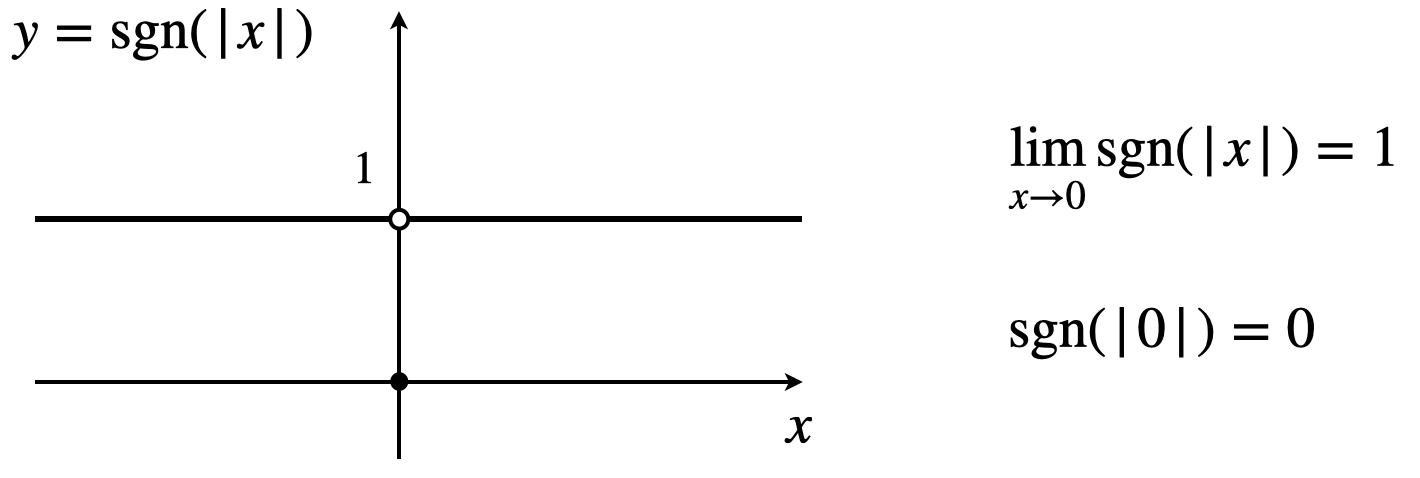
\includegraphics[width=90mm]{sgn_abs.png}
 \end{center}
\end{figure}

\vspace{-1mm}


\end{frame}


%%%%%%%%%%%%%%%%%%%%%%%%%%%%%%%%%%%%%%%%%%%%%%%%%%%%%%%%%%%%%%%%%%%%%%%%%%%%%%%%%%%%%%%
%%%%%%%%%%%%%%%%%%%%%%%%%%%%%%%%%%%%%%%%%%%%%%%%%%%%%%%%%%%%%%%%%%%%%%%%%%%%%%%%%%%%%%%


\begin{frame}
\frametitle{連続関数の直感} 


関数$f(x)$が$a$において連続とは, $f(x)$のグラフが$(a,f(a))$で繋がっているという直感を持てば良い. 



 \begin{figure}[htbp]
 \begin{center} 
  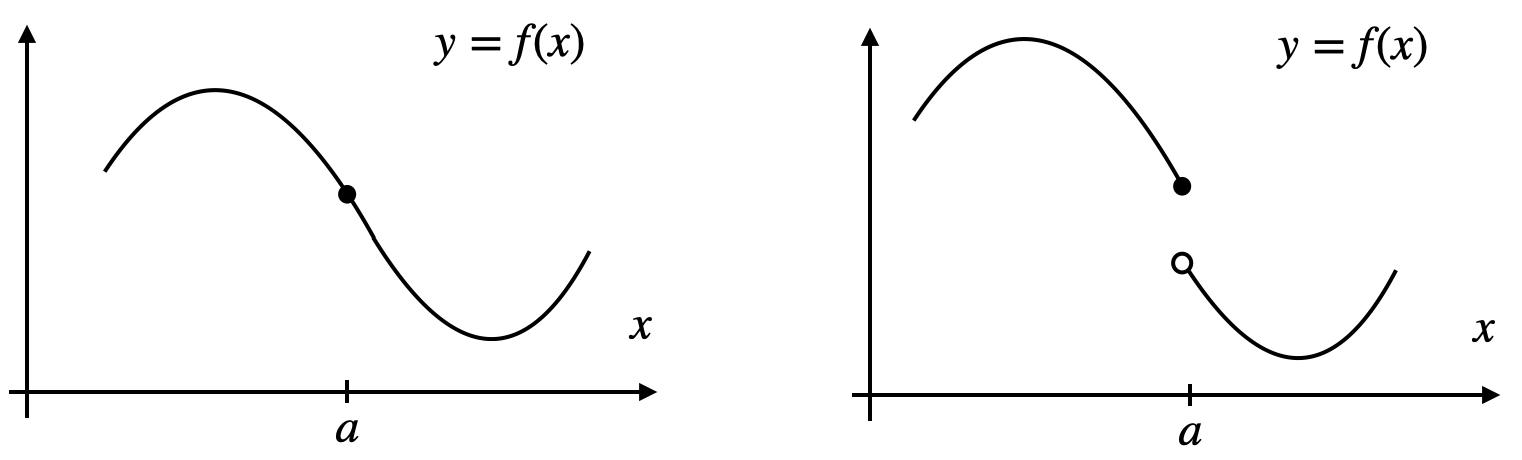
\includegraphics[width=100mm]{(dis)conti.png}
 \end{center}
\end{figure}

左図の関数は$a$で連続, 右図の関数は$a$で不連続. 
連続関数とは, グラフが(定義域において)繋がっている, 左図のような関数. 

\end{frame}



%%%%%%%%%%%%%%%%%%%%%%%%%%%%%%%%%%%%%%%%%%%%%%%%%%%%%%%%%%%%%%%%%%%%%%%%%%%%%%%%%%%%%%%
%%%%%%%%%%%%%%%%%%%%%%%%%%%%%%%%%%%%%%%%%%%%%%%%%%%%%%%%%%%%%%%%%%%%%%%%%%%%%%%%%%%%%%%


\begin{frame}
\frametitle{連続} 



\begin{Prob}
次の関数のグラフを描け. またこれらは連続関数か? 
\begin{itemize}
\item  $|x(x+3)(x-2)|$, 
\item  $\mathrm{sgn}(\sin x)$ 
\end{itemize}
\end{Prob}


\end{frame}


%%%%%%%%%%%%%%%%%%%%%%%%%%%%%%%%%%%%%%%%%%%%%%%%%%%%%%%%%%%%%%%%%%%%%%%%%%%%%%%%%%%%%%%
%%%%%%%%%%%%%%%%%%%%%%%%%%%%%%%%%%%%%%%%%%%%%%%%%%%%%%%%%%%%%%%%%%%%%%%%%%%%%%%%%%%%%%%


\begin{frame}
\frametitle{連続関数の加減乗除} 


\begin{Thm}
$f(x )$, $g(x)$が$a$において連続であるとする. 
\begin{itemize}
\item $cf(x)$, $f(x)+g(x)$, $f(x)g(x)$は$a$において連続. 
\item $g(a) \neq0$であれば, $f(x)/g(x)$は$a$において連続. 
\end{itemize}
\end{Thm}

\begin{itemize}
\item 恒等関数$f(x)=x$が連続関数であることから, 多項式関数や有理関数も(定義域において)連続関数である.  
\item 三角関数, 指数関数, 対数関数は連続関数であることが知られているため, $2\sin x -3 \log x$や$e^x \cos x$なども連続関数. 
\end{itemize}
\end{frame}


%%%%%%%%%%%%%%%%%%%%%%%%%%%%%%%%%%%%%%%%%%%%%%%%%%%%%%%%%%%%%%%%%%%%%%%%%%%%%%%%%%%%%%%
%%%%%%%%%%%%%%%%%%%%%%%%%%%%%%%%%%%%%%%%%%%%%%%%%%%%%%%%%%%%%%%%%%%%%%%%%%%%%%%%%%%%%%%


\begin{frame}
\frametitle{合成関数の連続性} 


\begin{Thm}
関数$f(x)$, $g(x)$に関して, 関数$f(x)$の定義域は$g(a)$を含み, 関数$g(x)$は$a$において連続であり, 
関数$f(x)$は$g(a)$において連続である時, 合成関数$f(g(x))$も$a$において連続. 
\end{Thm}

例: 次の関数は連続関数
$$
\sin(x^3+5x+2), \ \ \ e^{x^3}+\log(x^2+1), \ \ \ 
$$
他にも, $\log(x+1)$は$x\le-1$で定義されないが, $x>-1$において連続. 


\end{frame}



%%%%%%%%%%%%%%%%%%%%%%%%%%%%%%%%%%%%%%%%%%%%%%%%%%%%%%%%%%%%%%%%%%%%%%%%%%%%%%%%%%%%%%%
%%%%%%%%%%%%%%%%%%%%%%%%%%%%%%%%%%%%%%%%%%%%%%%%%%%%%%%%%%%%%%%%%%%%%%%%%%%%%%%%%%%%%%%


\begin{frame}
\frametitle{中間値の定理} 

連続関数に関する最も重要な定理が, 次の中間値の定理である. 

\begin{Thm}[中間値の定理]
関数$f(x)$が閉区間$[a,b]$で連続とする. 
$f(a) <  f(b)$を満たすとき, 任意の$l \in [f(a), f(b)]$に対して, $l=f(c)$なる点$c \in [a,b]$が存在する. 
\end{Thm}

 \begin{figure}[htbp]
 \begin{center} 
  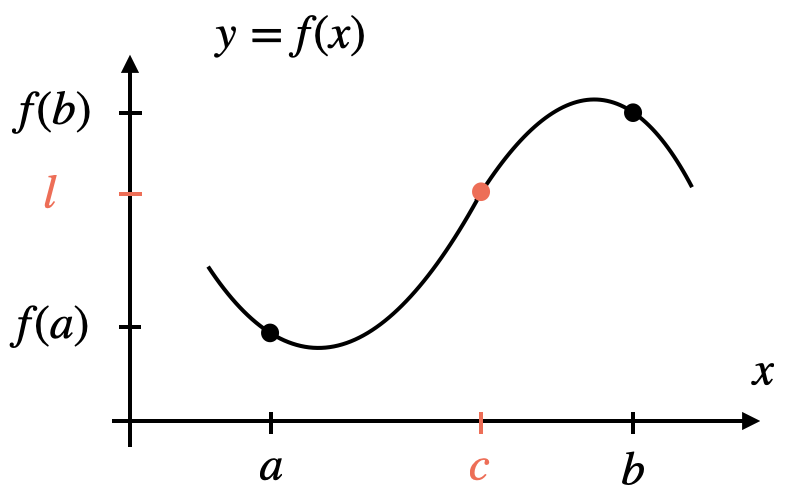
\includegraphics[width=60mm]{mean_value.png}
 \end{center}
\end{figure}


\end{frame}

%%%%%%%%%%%%%%%%%%%%%%%%%%%%%%%%%%%%%%%%%%%%%%%%%%%%%%%%%%%%%%%%%%%%%%%%%%%%%%%%%%%%%%%
%%%%%%%%%%%%%%%%%%%%%%%%%%%%%%%%%%%%%%%%%%%%%%%%%%%%%%%%%%%%%%%%%%%%%%%%%%%%%%%%%%%%%%%


\begin{frame}
\frametitle{極限計算} 



定義より, 関数が連続な点に関しては, 極限値を単に代入することで求めることができる. \\
\ \\

例えば, $(x^2+2x-3)/(x^2-1)$は$x\neq \pm1$において連続であるから, 
$$
\lim_{x \to 3} \frac{x^2+2x-3}{x^2-1}=\frac{3^2+2\cdot 3-3}{3^2-1}=\frac{3}{2}. 
$$
一方で, $1$は$(x^2+2x-3)/(x^2-1)$の定義域に入っていないため, この点において$f(x)$は連続でない. 
無理に代入すると
$$
\lim_{x \to 1} \frac{x^2+2x-3}{x^2-1}=\frac{1^2+2\cdot 1-3}{1^2-1}=\frac{0}{0} \ \ ?? 
$$
\end{frame}



%%%%%%%%%%%%%%%%%%%%%%%%%%%%%%%%%%%%%%%%%%%%%%%%%%%%%%%%%%%%%%%%%%%%%%%%%%%%%%%%%%%%%%%
%%%%%%%%%%%%%%%%%%%%%%%%%%%%%%%%%%%%%%%%%%%%%%%%%%%%%%%%%%%%%%%%%%%%%%%%%%%%%%%%%%%%%%%


\begin{frame}
\frametitle{極限計算} 



一方で, $1$は$(x^2+2x-3)/(x^2-1)$の定義域に入っていなくても, 
\begin{align*}
\lim_{x \to 1} \frac{x^2+2x-3}{x^2-1} &= \lim_{x \to 1} \frac{(x-1)(x+3)}{(x-1)(x+1)} \\
& = \lim_{x \to 1} \frac{x+3}{x+1} \\
& =  \frac{1+3}{1+1} =2 
\end{align*}

\begin{itemize}
\item 2つ目の等号: $x \to 1$において$x-1\neq 0$であるから, 分母分子を$x-1$で割ることができる. 
\item 3つ目の等号: 連続関数なので代入して極限を求めることが可能. 
\end{itemize}


\end{frame}



%%%%%%%%%%%%%%%%%%%%%%%%%%%%%%%%%%%%%%%%%%%%%%%%%%%%%%%%%%%%%%%%%%%%%%%%%%%%%%%%%%%%%%%
%%%%%%%%%%%%%%%%%%%%%%%%%%%%%%%%%%%%%%%%%%%%%%%%%%%%%%%%%%%%%%%%%%%%%%%%%%%%%%%%%%%%%%%


\begin{frame}
\frametitle{不定形} 

一般に, $\frac{0}{0}$, $\frac{\infty}{\infty}$, $\infty - \infty$といった形は\underline{不定形}と呼ばれる. 
特別な場合にはこれらは数学的に意味を持ち, 具体的に計算可能. 
次のような例がある. 

\begin{itemize}
\item $\displaystyle \lim_{x\to 2} \frac{x^2-x-2}{x^3-8}$
%\item $\displaystyle \lim_{x\to 3} \frac{x^3+x^2-14x+6}{x^2-9}$
\item $\displaystyle \lim_{x\to 0} \frac{1}{x}(1+\frac{1}{x-1})$
\item $\displaystyle \lim_{x \to \infty}\frac{4x^3-2x^2-10}{7x^3+5x+2}$
\item $\displaystyle \lim_{x\to -\infty} (3x^3+2x^2)$
\item $\displaystyle \lim_{x\to \infty} (\sqrt{x+100}-\sqrt{x})$
\end{itemize}


\end{frame}


%%%%%%%%%%%%%%%%%%%%%%%%%%%%%%%%%%%%%%%%%%%%%%%%%%%%%%%%%%%%%%%%%%%%%%%%%%%%%%%%%%%%%%%
%%%%%%%%%%%%%%%%%%%%%%%%%%%%%%%%%%%%%%%%%%%%%%%%%%%%%%%%%%%%%%%%%%%%%%%%%%%%%%%%%%%%%%%


\begin{frame}
\frametitle{不定形} 


\begin{align*}
\lim_{x\to 2} \frac{x^2-x-2}{x^3-8}
& =  \lim_{x\to 2} \frac{(x-2)(x+1)}{(x-2)(x^2+2x+4)} \\
& =   \lim_{x\to 2}\frac{x+1}{x^2+2x+4} \\
& = \frac{3}{12}=\frac{1}{4} \\
\ & \ \\
\lim_{x\to 0} \frac{1}{x}(1+\frac{1}{x-1})
& =  \lim_{x\to 0} \frac{1}{x} \frac{x}{x-1} \\
& =  \lim_{x\to 0}\frac{1}{x-1} \\
& = -1
\end{align*}


%\begin{align*}
%\lim_{x\to 3} \frac{x^3+x^2-14x+6}{x^2-9}
%& =  \lim_{x\to 3} \frac{(x-3)(x^2+4x-2)}{(x+3)(x-3)} \\
% & =  \lim_{x\to 3} \frac{x^2+4x-2}{x+3} \\
% & = \frac{19}{6}. 
%\end{align*}


\end{frame}


%%%%%%%%%%%%%%%%%%%%%%%%%%%%%%%%%%%%%%%%%%%%%%%%%%%%%%%%%%%%%%%%%%%%%%%%%%%%%%%%%%%%%%%
%%%%%%%%%%%%%%%%%%%%%%%%%%%%%%%%%%%%%%%%%%%%%%%%%%%%%%%%%%%%%%%%%%%%%%%%%%%%%%%%%%%%%%%


\begin{frame}
\frametitle{不定形} 


\begin{align*}
\lim_{x \to \infty}\frac{4x^3-2x^2-10}{7x^3+5x+2} 
& = \lim_{x \to \infty} \frac{4-\frac{2}{x}-\frac{10}{x^3}}{7+\frac{5}{x^2}+\frac{2}{x^3}} = \frac{4}{7}. \\
\ & \ \\
\lim_{x\to -\infty} (3x^3+2x^2)
& =  \lim_{x\to -\infty} x^3(3+\frac{2}{x})  = -\infty
\end{align*}


\end{frame}


%%%%%%%%%%%%%%%%%%%%%%%%%%%%%%%%%%%%%%%%%%%%%%%%%%%%%%%%%%%%%%%%%%%%%%%%%%%%%%%%%%%%%%%
%%%%%%%%%%%%%%%%%%%%%%%%%%%%%%%%%%%%%%%%%%%%%%%%%%%%%%%%%%%%%%%%%%%%%%%%%%%%%%%%%%%%%%%


\begin{frame}
\frametitle{不定形} 


\begin{align*}
\lim_{x\to \infty} (\sqrt{x+100}-\sqrt{x})
& =  \lim_{x\to \infty} \frac{(\sqrt{x+100}-\sqrt{x})(\sqrt{x+100}+\sqrt{x})}{\sqrt{x+100}+\sqrt{x}} \\
& =  \lim_{x\to \infty} \frac{100}{ \sqrt{x+100}+\sqrt{x}} \\
& =0
\end{align*}


\end{frame}






%%%%%%%%%%%%%%%%%%%%%%%%%%%%%%%%%%%%%%%%%%%%%%%%%%%%%%%%%%%%%%%%%%%%%%%%%%%%%%%%%%%%%%%
%%%%%%%%%%%%%%%%%%%%%%%%%%%%%%%%%%%%%%%%%%%%%%%%%%%%%%%%%%%%%%%%%%%%%%%%%%%%%%%%%%%%%%%




\section{今日のまとめ}
\begin{frame}
\frametitle{まとめ}   


\begin{enumerate}
\item 極限 (右極限, 左極限, 極限, 極限の性質)
\item 連続 (点連続, 連続関数, 中間値の定理)
\item 不定形の極限
\end{enumerate} 


\end{frame}


\end{document}